\section{Algorytm rozpoznawania znaków}
Segmentacja obrazu prowadzi do wyodrębnienia z obrazu żądanych obiektów. Zwykle jest ona pierwszym etapem analizy całego obrazu. Odnalezione obiekty bardzo często poddawane są analizie w celu identyfikacji lub podjęcia decyzji.
\paragraph{}
W przypadku problemu rozpoznawania znaków, zadaniem algorytmu segmentacji jest określenie lokalizacji każdego znaku oraz binaryzacja fragmentów obrazu zawierającego tekst. Kolejnym krokiem jest dostarczenie serii wykadrowanych obrazów binarnych zawierających pojedyncze znaki do algorytmu rozpoznawania znaków. Zadaniem algorytmu rozpoznawania znaków jest określenie, jaki znak tekstu znajduje się na zadanym obrazie.
\paragraph{}
Poniżej zostanie opisanych kilka algorytmów rozpoznawania znaków.
\subsection{Cechy geometryczne}
Zestaw cech geometrycznych jest unikalny dla każdego znaku, dlatego sprawdzając odpowiednie warunki, można określić jego dokładne znaczenie. Właściwości geometryczne znaków zostały obszernie opisane w publikacji \cite{frey91}. Poniżej znajduje się lista wybranych cech geometrycznych, które mogą być brane pod uwagę podczas rozpoznawania znaków.
\begin{itemize}
  \item wysokość oraz szerokość prostokąta otaczającego znak
  \item stosunek liczby punktów należących do znaku do liczby punktów stanowiących tło
  \item stosunek liczby punktów należących do znaku i znajdujących się w górnej połówce obrazu, do liczby punktów należących do znaku i znajdujących się w dolnej połówce obrazu
    \item stosunek liczby punktów należących do znaku i znajdujących się w lewej połówce  obrazu, do liczby punktów należących do znaku i znajdujących się w prawej połówce obrazu
    \item liczba pionowych oraz poziomych krawędzi znaku
\end{itemize}
\subsection{Rzut jasności obiektu}
Metoda rzutu jasności obiektu została opisana na stronie~\pageref{ssec:rzut_jasnosci}. W pierwszej kolejności należy przeskalować obraz do rozmiarów obrazu wzorcowego, a następnie wykonać algorytm rzutu jasności zarówno w pionie, jak i w poziomie. Otrzymane rzuty zostają następnie poddane analizie podobieństwa z rzutami wykonanymi dla znaków wzorcowych. Analiza podobieństwa polega na porównaniu kształtu otrzymanych rzutów jasności. \\
Na rysunku~\ref{fig:rzut_jasnosci_ocr} przedstawione zostały wzorce kilku znaków, oraz przykładowy obraz wejściowy.

\begin{figure}
  \centering
  \begin{subfigure}[b]{0.42\textwidth}
    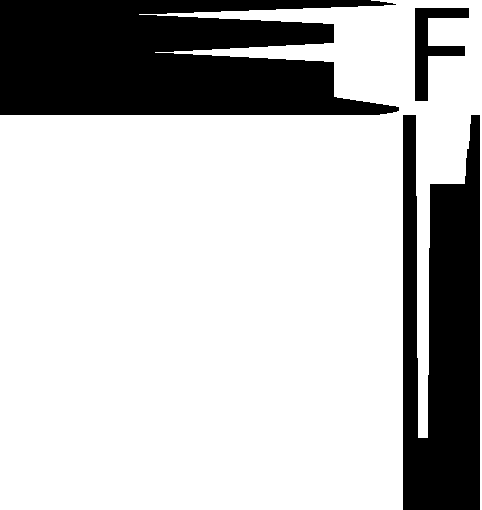
\includegraphics[width=\textwidth]{img/rzut-wzorzec-F}
    \caption{Wzorzec dla litery F}
    \label{fig:rzut_wzorzec_F}
  \end{subfigure}
  ~
  \begin{subfigure}[b]{0.42\textwidth}
    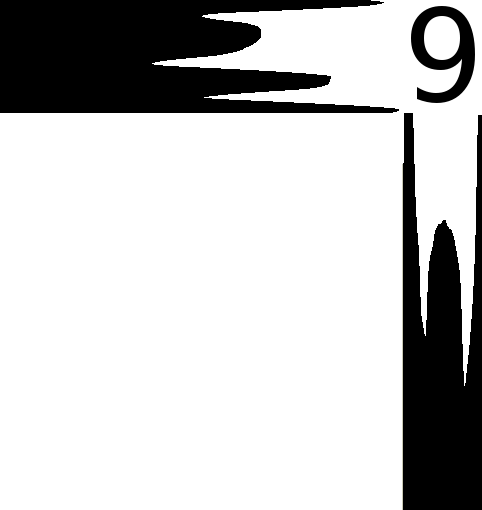
\includegraphics[width=\textwidth]{img/rzut-wzorzec-9}
    \caption{Wzorzec dla cyfry 9}
    \label{fig:rzut_wzorzec_9}
  \end{subfigure}
  \begin{subfigure}[b]{0.44\textwidth}
    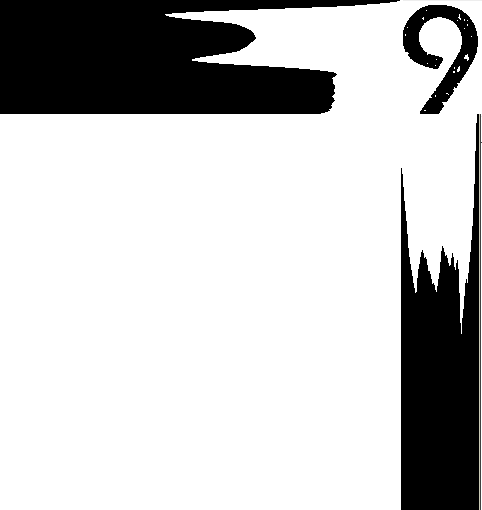
\includegraphics[width=\textwidth]{img/rzut-in-9}
    \caption{Obraz wejściowy, zawierający cyfrę 9}
    \label{fig:rzut_in_9}
  \end{subfigure}
  \caption{Porównanie rzutu jasności dla wybranych znaków}
    \label{fig:rzut_jasnosci_ocr}
\end{figure}

\subsection{Sztuczne sieci neuronowe}
Sztuczne sieci neuronowe(SSN) to struktury tworzone na podobieństwo biologicznych sieci neuronowych \cite{tadeusiewicz93}. SSN mają zdolność do uogólniania zdobytej wiedzy. Podobnie jak w przypadku biologicznych, w sztucznych sieciach neuronowych podstawowym elementem są neurony, które połączone są miedzy sobą za pomocą synaps. Każda synapsa posiada parametr zwany wagą, który jest modyfikowany w poszczególnych fazach uczenia sieci neuronowej. Sieci neuronowe zorganizowane są w strukturze wielowarstwowej:
\begin{itemize}
  \item warstwa wejściowa,
  \item warstwy ukryte,
  \item warstwa wyjściowa.
\end{itemize}
W zależności od złożoności problemu, sieć neuronowa może zawierać różną liczbę neuronów w każdej warstwie, oraz różną liczbę warstw ukrytych. Przykład SSN można znaleźć na rysunku~\ref{fig:ssn_example}. Wartość wyjściowa neuronu wyznaczana jest na podstawie sygnałów wejściowych oraz funkcji aktywacji. Dla każdego neuronu wartość wyjściowa wyznaczana jest za pomocą wzoru:
\begin{gather*}
  y = g(\sum_{i=1}^{N}w_ix_i+w_0),
\end{gather*}
gdzie:\\
$g$ - funkcja aktywacji,\\
$N$ - liczba wejść poprzedniej warstwy,\\
$w_i$ - waga synapsy i-tego sygnału,\\
$x_i$ - wartość i-tego sygnału.\\
W zależności od wybranego algorytmu, sieć poddawana jest procesowi uczenia, podczas którego wartości wag $w_i$ są korygowane.\\
Jako zestaw uczący, a następnie zestaw testowy, podawane mogą być obrazy ze znakami. Po wykonaniu procesu uczenia, sieć neuronowa powinna mieć zdolność do dopasowania obrazu do najlepszego wyuczonego wzorca. 
\begin{figure}
  \centering
  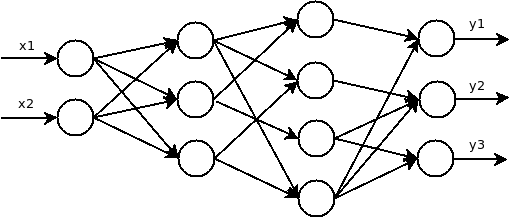
\includegraphics[width=10cm]{img/ssn-example}
  \caption{Przykładowa sieć neuronowa, zawierająca dwa neurony w warstwie wejściowej, dwie warstwy ukryte, oraz warstwę wejściową zawierającą trzy neurony.}
  \label{fig:ssn_example}
\end{figure}
